\documentclass[11pt]{article}
\usepackage{a4wide}
\usepackage{amsmath}
\usepackage{amssymb}
\usepackage{amsthm}
\usepackage{bbm}
\usepackage{cite}
\usepackage{subfig}
\usepackage{graphicx}
\usepackage{hyperref}
\usepackage{color}
\usepackage{xspace}
\usepackage[ruled, noline, algo2e, noend, linesnumbered]{algorithm2e}

\newcommand{\todo}[1]{\xspace{\bfseries\sffamily\textcolor{red}{[#1]}}\xspace}

\newtheorem{problem}{Problem}[section]
\newtheorem{definition}{Definition}[section]
\newtheorem{theorem}{Theorem}[section]
\newtheorem{lemma}[theorem]{Lemma}
\newtheorem{proposition}[theorem]{Proposition}
\newtheorem{corollary}[theorem]{Corollary}

\author{M.~El-Kebir \and  G.~W.~Klau}
\title{Fragment-based molecule parameterization}

\begin{document}

\maketitle

\section{Introduction}

The automated topology builder (ATB) is a web server for generating topologies
of novel molecules compatible with the GROMOS 53A6 force field \cite{Malde11}.
The ATB is able to parameterize molecules consisting of up to 50 atoms. Due to
the complexity of the quantum mechanics computations, molecules larger than 50
atoms pose a problem for the ATB.

Here, we introduce a method that assists the ATB by searching for fragments
common to both the input molecule and a molecule in the repository. The atom
charges of the input molecule are set according to the charges of the core atoms
of the found common fragments.

\section{Problem definition}

A molecular graph is a simple graph $G=(V,E)$ whose nodes and edges correspond
to atoms and bonds, respectively. Nodes are labeled by their partial charge $w :
V \rightarrow \mathbb{R}$ and their atom type $t : V \rightarrow T$ where $T$ is
the set of all atom types. For a subset $V^\prime \subseteq V$, $t(V^\prime)$ is the
set $\bigcup_{v \in V^\prime} t(v)$, i.e.\ $t(V^\prime)$ is the set of all atom
types of nodes in $V^\prime$.

\begin{definition}
  The \emph{$i$-neighborhood} of a node $v \in V$ is defined recursively as
  \[
    N^i(v) = 
  \begin{cases}
    \emptyset, & \mbox{if $i=0$,}\\
    \{ u \mid (u,v) \in E \}, & \mbox{if $i=1$,}\\
    N^{i-1}(v) \cup \{ u \mid (u,w) \in E, w \in N^{i-1}(v), u \not \in
    N^{i-1}(v) \}, & \mbox{if $i > 1$.}
  \end{cases}
  \]
  For a subset $V^\prime \subseteq V$, we define $N^i(V^\prime)$ to
  be the set $\bigcup_{v \in V^\prime} N^i(v) \setminus V^\prime$.
\end{definition}

Given molecules $G_1 = (V_1, E_1)$ and $G_2 = (V_2, E_2)$ with atom types $t_1 :
V_1 \rightarrow \mathbb{N}$ and $t_2 : V_2 \rightarrow \mathbb{N}$ and $k \in
\mathbb{N}$, we define a $k$-common fragment and its shell as follows.

\begin{definition}
Given $k \in \mathbb{N}$, a \emph{$k$-common fragment} is a pair $(V^\prime_1,
V^\prime_2)$ with $V^\prime_1 \subseteq V_1$ and $V^\prime_2 \subseteq V_2$ that
admits a bijection $h : V^\prime_1 \cup N^k(V^\prime_1) \rightarrow V^\prime_2
\cup N^k(V^\prime_2)$ such that
\begin{enumerate}
  \item[(i)] $G_1[V^\prime_1]$ and $G_2[V^\prime_2]$ are connected,
  \item[(ii)] $(u,v)$ is an edge in $G_1[V^\prime_1 \cup N^k(V^\prime_1)]$ if and
    only if $(h(u),h(v))$ is an edge in ${G_2[V^\prime_2 \cup
    N^k(V^\prime_2)]}$,
  \item[(iii)] $t_1(v) = t_2(h(v))$ for all $v \in V^\prime_1 \cup
    N^k(V^\prime_1)$.
\end{enumerate}
\end{definition}

\begin{definition}
The \emph{shell} of a $k$-common fragment $(V^\prime_1, V^\prime_2)$ is given by
$(N^k(V^\prime_1), N^k(V^\prime_2))$.
\end{definition}

\begin{definition}
A $k$-common fragment $(V^\prime_1,V^\prime_2)$ is \emph{maximal} if there
exists no $k$-common fragment $(V^{\prime\prime}_1,V^{\prime\prime}_2)$ such
that $V^\prime_1 \subseteq V^{\prime\prime}_1$ and $V^\prime_2 \subseteq
V^{\prime\prime}_2$.
\end{definition}

The problem that we want to solve is now as follows. See
Figure~\ref{fig:example} for an example.

\begin{problem}
Given graphs $G_1 = (V_1, E_1)$ and $G_2 = (V_2, E_2)$ with atom types $t_1 :
V_1 \rightarrow \mathbb{N}$ and $t_2 : V_2 \rightarrow T$ and $k \in
\mathbb{N}$, find the set of all maximal $k$-common fragments.
\end{problem}

\begin{figure}
  \center
  \subfloat[\label{fig:16481}$G_1$]{%, the 1-neighborhood of the green and the red
  %  subgraphs consists of C1 and C2, respectively.]{
      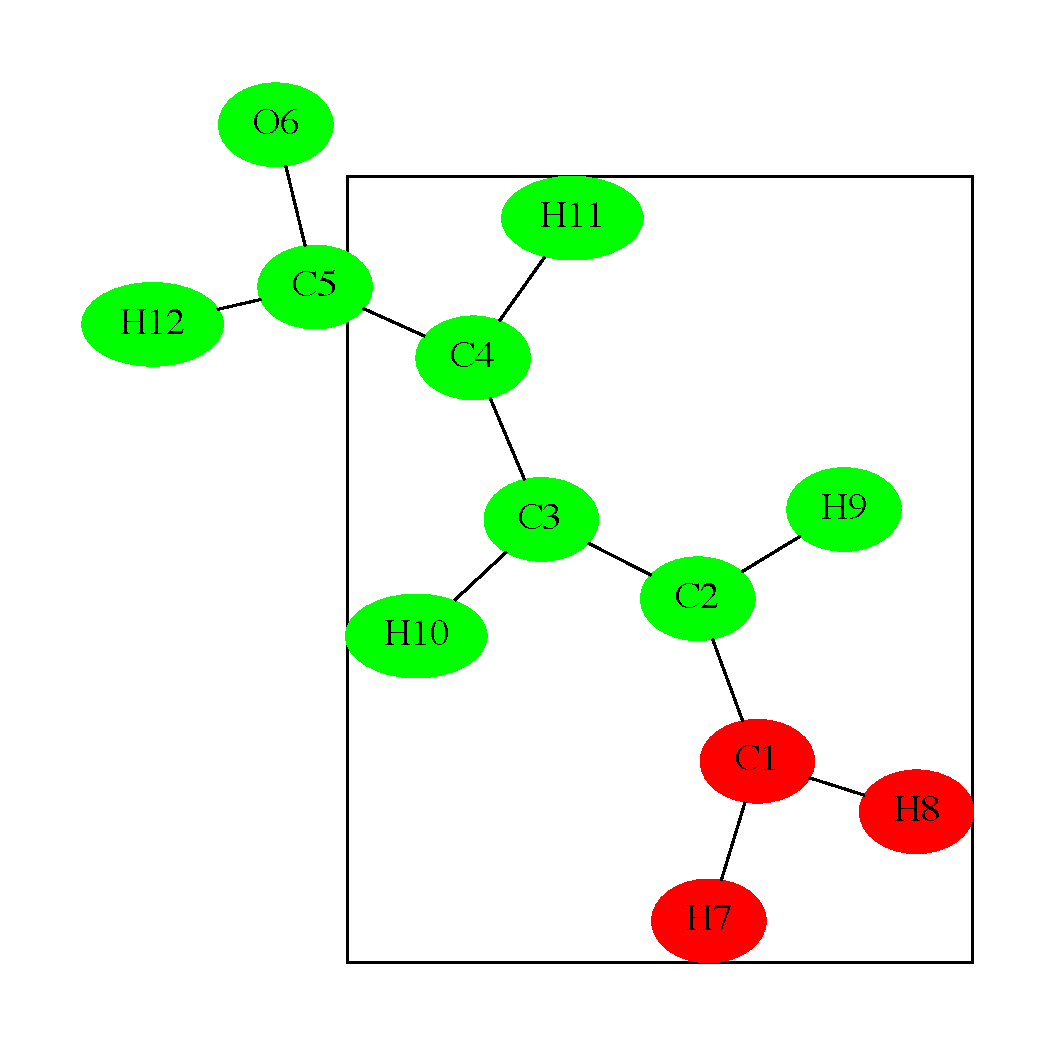
\includegraphics[scale=.35]{images/16841.pdf}
  }
  \subfloat[\label{fig:16482}$G_2$]{%, the 1-neighborhood of the green and the red
  %  subgraphs consists of C3 and C2, respectively.]{
      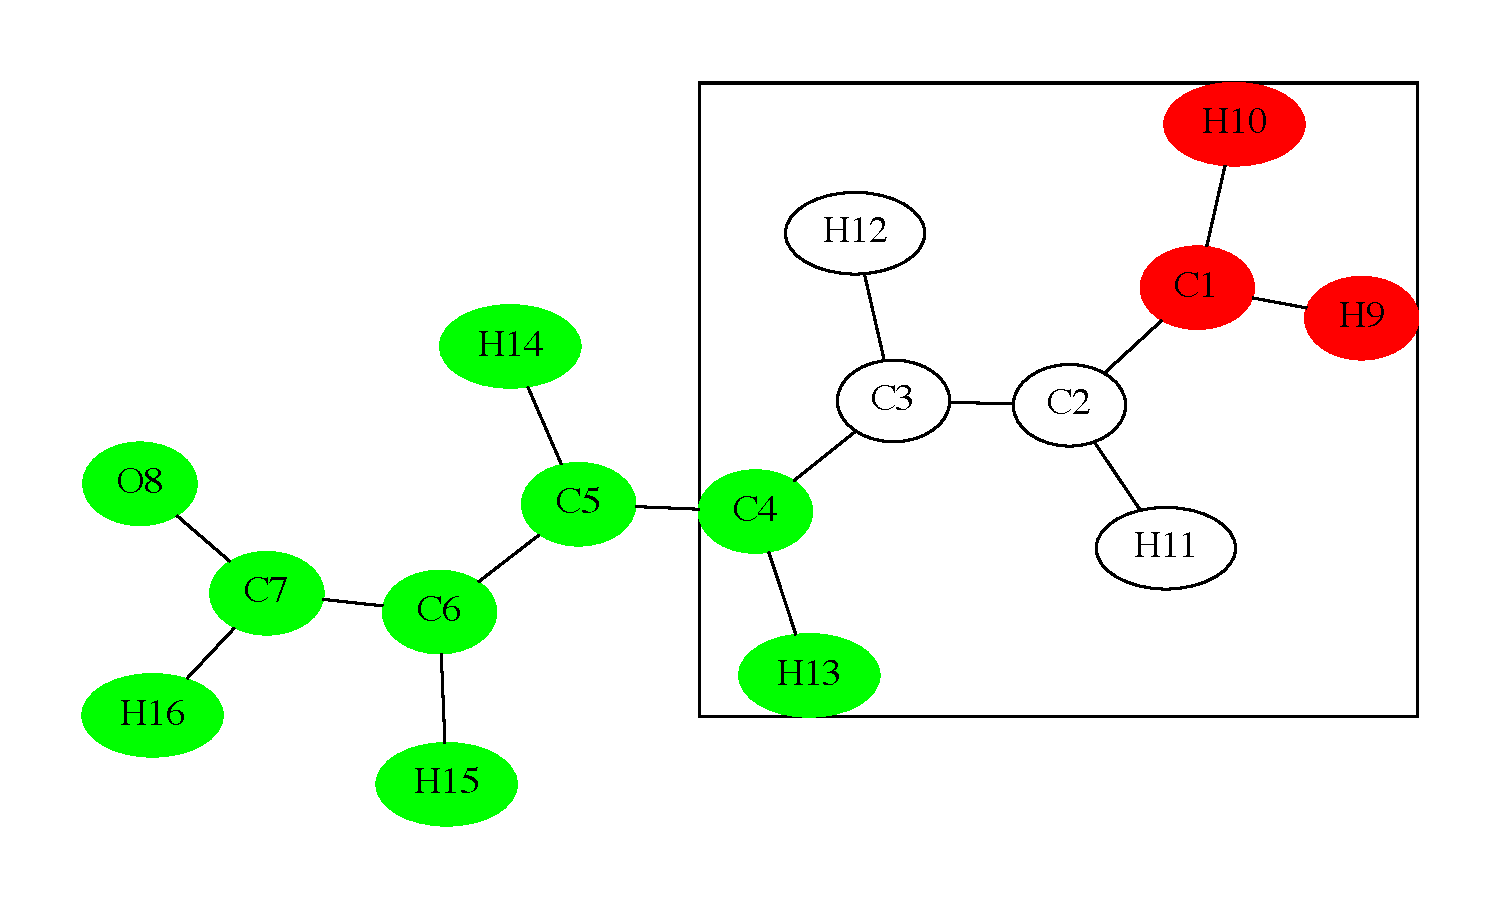
\includegraphics[scale=.35]{images/16842.pdf}
  }
  \\
  \subfloat[Maximal common fragments]{
    \centering
    \small
    \begin{tabular}{|l|p{.8\textwidth}|}
      \hline
      1 & (C4~,~C5), (H11~,~H14), (C3~,~C6), (H10~,~H15)\\
      2 & (C3~,~C6), (H10~,~H15), (C2~,~C5), (H9~,~H14)\\
      3 & (C4~,~C3), (H11~,~H12), (C3~,~C2), (H10~,~H11)\\
      4 & (C3~,~C2), (H10~,~H11), (C2~,~C3), (H9~,~H12)\\
      5 & (C4~,~C3), (H11~,~H12), (C3~,~C4), (H10~,~H13), (C2~,~C5), (H9~,~H14)\\
      6 & (C4~,~C4), (H11~,~H13), (C3~,~C5), (H10~,~H14), (C2~,~C6), (H9~,~H15)\\
      7 & (C4~,~C2), (H11~,~H11), (C3~,~C3), (H10~,~H12), (C2~,~C4), (H9~,~H13)\\
      8 & (C4~,~C5), (H11~,~H14), (C3~,~C4), (H10~,~H13), (C2~,~C3), (H9~,~H12)\\
      9 & (C1~,~C1), (H7~,~H10), (H8~,~H9), (C4~,~C4), (H11~,~H13), (C3~,~C3), (H10~,~H12), (C2~,~C2), (H9~,~H11)\\
      10 & (C5~,~C7), (H12~,~H16), (O6~,~O8), (C4~,~C6), (H11~,~H15), (C3~,~C5), (H10~,~H14), (C2~,~C4), (H9~,~H13)\\
      \hline
    \end{tabular}
  }
  \caption{There are ten maximal 1-common fragments. The last row corresponds to
    the fragments colored in green. Observe that the 1-neighborhood of the green
    fragment in $G_1$ consists of C1 and in $G_2$ it consists of C3, both of
    which have the same atom type (C). The red fragments are 1-common fragments,
    but are not maximal---they are each contained within a larger 1-common
    fragment as shown by the boxes.}
  \label{fig:example}
\end{figure}

\subsection{Complexity}

\begin{lemma}
Enumerating all maximal $k$-common fragments is NP-hard.
\end{lemma}
\begin{proof}
  We show by reduction from the induced subgraph isomorphism problem, which
  asks, given two graphs $G_1 = (V_1, E_1)$ and $G_2 = (V_2, E_2)$ with $|V_1|
  \leq |V_2|$, whether $G_1$ is an induced subgraph of $G_2$---i.e., whether 
  there exists an injective function $f : V_1 \rightarrow V_2$ such that $(u,v)
  \in E_1$ if and only if $(f(u),f(v)) \in E_2$.

  We obtain the corresponding $k$-common fragments problem by using the same
  graphs $G_1$ and $G_2$, choosing $T = \mathbbm{1}$, and setting $k = 0$. Now
  we claim that $G_1$ is an induced subgraph of $G_2$ if and only if $G_1$ and
  $G_2$ have a 0-common fragment of size $|V_1|$. \todo{Finish proof, trivial.}
\end{proof}

\section{Related work}

\begin{itemize}
  \item \todo{Talk about maximum common subgraph isomorphisms
    algorithms~\cite{Raymond:2002ug}}
  \item \todo{Talk about reducing MCIS to maximum clique problem in the product
    graph}
  \item \todo{Talk about the Bron-Kerbosch algorithm~\cite{Bron:1973tk}}
  \item \todo{Talk about the work of Ina Koch~\cite{Koch:2001wi}}
\end{itemize}

\section{Method}

We solve the problem by finding maximal cliques on the product graph, which is
defined as follows.

\begin{definition}
Given $k \in \mathbb{N}$, the \emph{$k$-product graph} $G_1 \otimes G_2 =
(V_{12}, E_{12})$ has node set $V_{12} = \{(u,v) \in V_1 \times V_2 \mid t_1(u)
= t_2(v), t_1(N^k(u)) = t_2(N^k(v)) \}$ and an edge in $E_{12}$ between $(u,v)$
and $(u^\prime,v^\prime)$ if and only if $u \neq u^\prime$ and $v \neq
v^\prime$, and either $(u,u^\prime) \in E_1$ and $(v,v^\prime) \in E_2$, or
$(u,u^\prime) \not \in E_1$ and $(v,v^\prime) \not \in E_2$.
\end{definition}

Following \cite{Koch:2001wi}, we distinguish between $c$ and $d$-edges in the
product graph.

\begin{definition}
An edge $((u,v),(u^\prime,v^\prime)) \in E_{12}$ is a \emph{$c$-edge} if
$(u,u^\prime) \in E_1$ and $(v,v^\prime) \in E_2$, otherwise it is a
\emph{$d$-edge}.
\end{definition}

The $c$-neighborhood $N_c(v)$ of a node $v \in V_{12}$ is the set $\{ u
\mid (u,v) \in E_{12}, (u,v) \mbox{ is a $c$-edge} \}$. Conversely, $N_d(v)$ is
the $d$-neighborhood of a node $v \in V_{12}$.
%Similarly for a subset $V^\prime_{12} \subseteq V_{12}$, we define $N_c(V^\prime)$ to be the set
%$\bigcup_{v \in V^\prime} N_c(v)$. 
Now we define a $c$-clique as follows.

\begin{definition}
A \emph{$c$-clique} $C \subseteq V_{12}$ is a clique in $G_{12}$ containing at
least one $c$-edge. \todo{g: this is not enough. spanning tree of $c$-edges?}
\end{definition}

\begin{definition}
A $c$-clique $C \subseteq V_{12}$ is \emph{maximal} if there is no
$c$-clique $C^\prime$ such that $C \subseteq C^\prime$.
\end{definition}

In order to ensure connectivity, we aim to find maximal $c$-cliques. Ina Koch
has shown that $c$-cliques correspond to $k$-common fragments with the same size.

\begin{lemma}
A $c$-clique $C$ in $G_{12}$ corresponds to a $k$-common fragment of size $|C|$.
\end{lemma}
\begin{proof}
See Ina Koch~\cite{Koch:2001wi}.
\end{proof}

\begin{figure}
  \center
  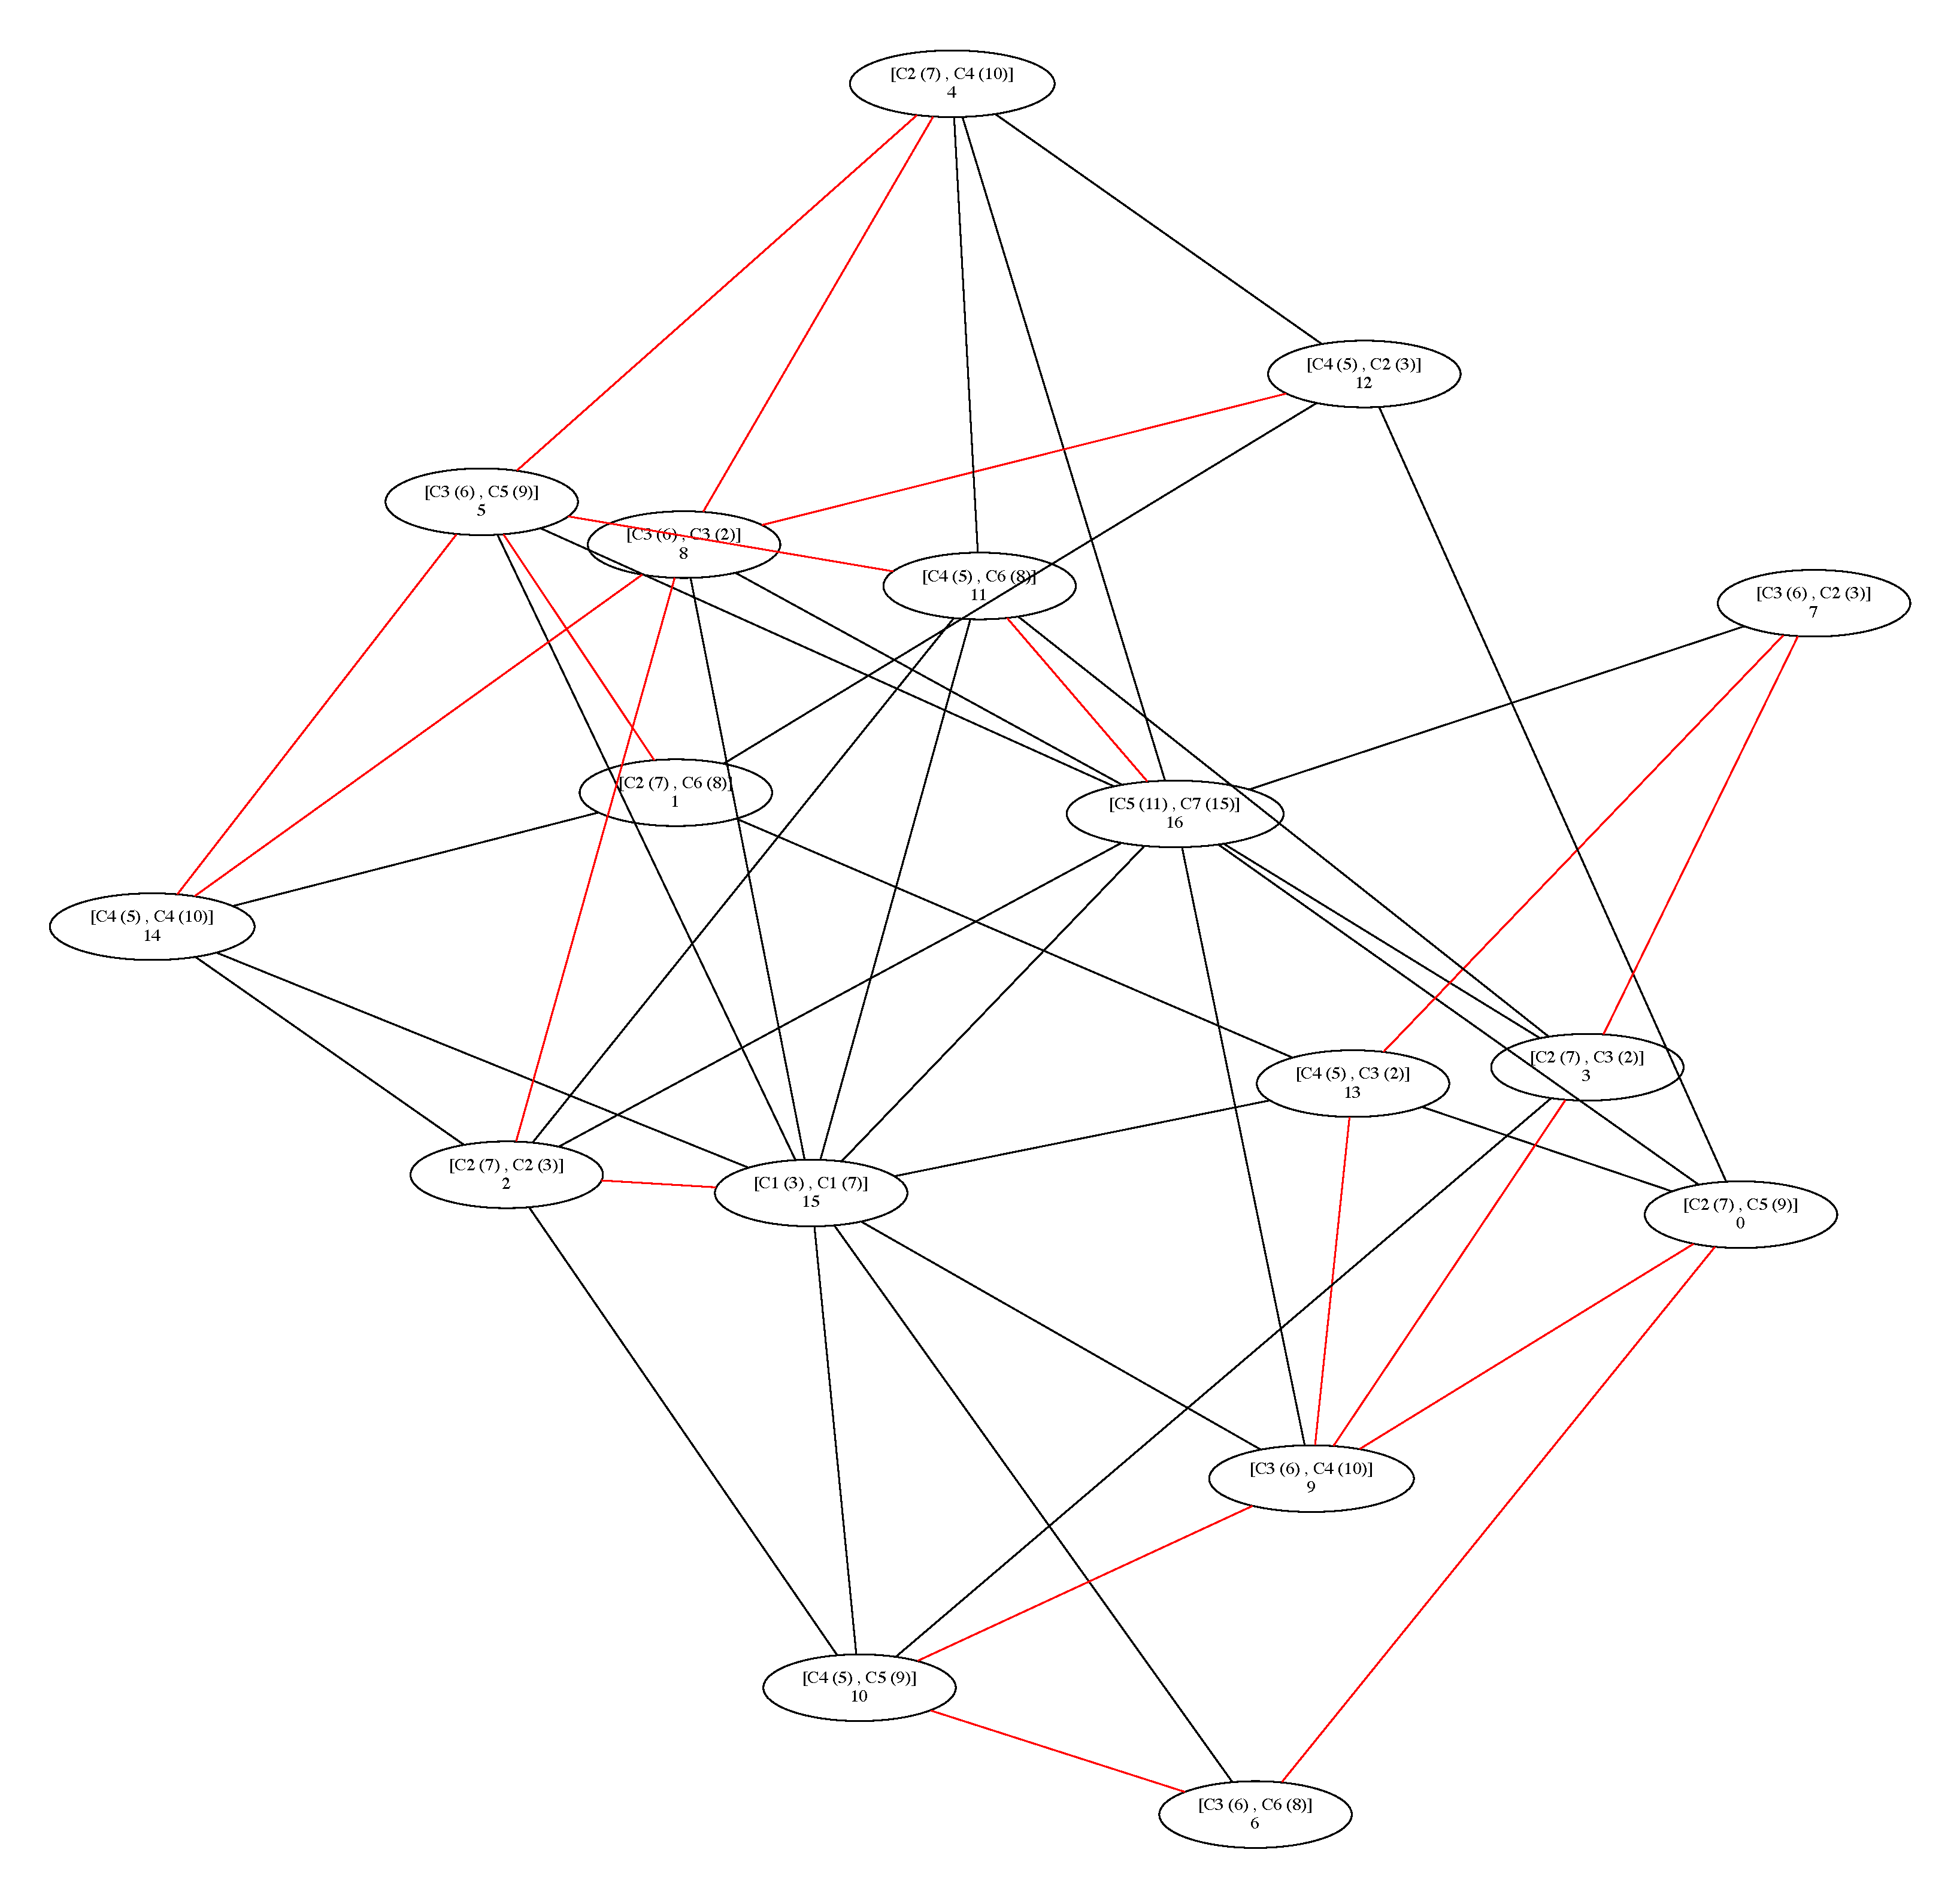
\includegraphics[width=1.1\textwidth]{images/product}
  \caption{The product graph; as an optimization product nodes corresponding to
    degree 1 nodes in the original graphs have been ignored. $c$-edges are
    colored red and $d$-edges are colored black. These are the maximal
    $c$-cliques: $\{10,6\}, \{10,0\}, \{13, 7\},
    \{7, 3\}, \{13, 9, 0\}, \{14, 5, 1\}, \{12, 8, 4\}, \{10, 9, 3\}, \{16, 11,
    5, 4\}$ and $\{15, 14, 8, 2\}$.}
  \label{fig:product}
\end{figure}

We identify maximal $c$-cliques by adapting Bron-Kerbosch' algorithm similarly
to~\cite{Koch:1996fc,Koch:2001wi}.

\begin{algorithm2e}
  \caption{\textsc{cCliques}$(P,D,R,X,S)$}
  \label{alg:bk-pivot}
  \KwIn{$P$, $D$, $X$ and $S$ are disjoint sets of nodes adjacent to all nodes
    in $R$ whose nodes induce a $c$-clique in $G_{12}$.}
    %All nodes in $P$ are $c$-adjacent to at least one node in $R$. All nodes in
    %$D$ are $d$-adjacent to all nodes in $R$. $R$ defines a maximal $c$-clique.}
  \If{$P \cup X = \emptyset$}{
    Report $R$
  }
  \Else{
    Choose $u \in P \cup X$ maximizing $|P \cap N(u)|$\\
    \ForEach{$v \in P \setminus N(u)$}{
      $P^\prime \leftarrow P \cup (D \cap N_c(v))$\\
      $D^\prime \leftarrow D \setminus N_c(v)$\\
      $X^\prime \leftarrow X \cup (S \cap N_c(v))$\\
      $S^\prime \leftarrow S \setminus N_c(v)$\\
      \textsc{BK}($P^\prime \cap N(v)$, $D^\prime  \cap N(v)$, $R \cup \{v\}$,
      $X^\prime \cap N(v)$, $S^\prime \cap N(v)$)\\
      $P \leftarrow P \setminus \{v\}$\\
      $X \leftarrow X \cup \{v\}$
    }
  }
\end{algorithm2e}

\begin{lemma}
There are five invariants in the algorithm.
\begin{enumerate}
  \item $R$ is a clique.
  \item Each node $v \in P$ is adjacent to all nodes in $R$ and $c$-adjacent to
    at least one node in $R$.
  \item Each node $v \in D$ is $d$-adjacent to all nodes in $R$.
  \item Each node $v \in X$ is adjacent to all nodes in $R$ and $c$-adjacent to
    at least one node in $R$, and all maximal
    $c$-cliques containing $R \cup \{v\}$ have already been reported.
  \item Each node $v \in S$ is $d$-adjacent to all nodes in $R$ and all maximal
    $c$-cliques containing $R \cup \{v\}$ have already been reported.
\end{enumerate}
\end{lemma}
\begin{proof}
\todo{Give proof}
\end{proof}

Invoking \textsc{cCliques}($P, D, R, X, S$) lists all maximal $c$-cliques in the
subgraph comprised of the nodes in $R$, some of the nodes in $P \cup D$
and none of the nodes in $X \cup S$. So by invoking \textsc{cCliques}($N_c(v),
N_d(v), \{ v \}, \emptyset, \emptyset$) all maximal $c$-cliques containing $v
\in V_{12}$ will be listed. In fact, the pivot rule we use (line~4,
Algorithm~\ref{alg:bk-pivot}) ensures that every maximal $c$-clique containing
$v$ is listed exactly once~\cite{Tomita:2006kb}. By considering the nodes in a
degeneracy ordering \cite{Eppstein:2010uq}, we can bound the size of $P \cup D$
and arrive at a worst-case running time of
$O(dn3^{d/3})$~\cite{Eppstein:2010uq}---see Algorithm~\ref{alg:bk-degeneracy}.
\todo{Maybe a tighter bound can be obtained.}

\begin{algorithm2e}
  \caption{\textsc{AllcCliques}$()$}
  \label{alg:bk-degeneracy}
  Let $v_1, v_2, \ldots, v_n$ be a degeneracy ordering\\
  \For{$i \leftarrow 1$ \KwTo $n$}
  {
    $P \leftarrow N_c(v_i) \cap \{v_{i+1}, \ldots, v_n\}$\\
    $D \leftarrow N_d(v_i) \cap \{v_{i+1}, \ldots, v_n\}$\\
    $X \leftarrow N_c(v_i) \cap \{v_1, \ldots, v_{i-1}\}$\\
    $S \leftarrow N_d(v_i) \cap \{v_1, \ldots, v_{i-1}\}$\\
    \textsc{BK}$(P, D, \{v_i\}, X, S)$
  }
\end{algorithm2e}

\section{Results}

We compiled a repository of fragments based on the lipid data set of the ATB. 
This set contains 151 molecules of sizes varying from 25 up to 285 atoms. 
The computation of all maximal common fragments between the molecule in 
Figure~\ref{fig:16481} and the 151 molecules in the repository takes 2 seconds. 
For larger molecules, such as the one with molecule id 6401 (145 atoms), 
enumerating all the maximal common fragments takes 2.5 minutes on a standard
desktop computer.

\section{Discussion}

Future work includes the following.
\begin{itemize}
  \item How to combine fragments? What about using exact cover, i.e., find a set
    of disjoint maximal common fragments that covers the input molecule?
  \item What is a good repository?
\end{itemize}

\bibliographystyle{abbrv}
\bibliography{fragments}

\end{document}

